\documentclass{seminar}
\usepackage{amsmath, amssymb, color, xcolor}
\usepackage{graphicx, wrapfig, float, caption, dsfont}
\usepackage{fullpage}
\usepackage[backref=page, hidelinks, colorlinks=true, citecolor=blue!60!black!100]{hyperref}
\usepackage{tikz}
\usetikzlibrary{arrows.meta, shapes, backgrounds}
\usepackage{caption, subcaption}
\usepackage{natbib} % gives us \citet: Author (year) and \citep: (Author; year)
\usepackage{authblk}

\newcommand{\plr}[1]{{\color{blue}\it #1}}
\newcommand{\jss}[1]{{\color{olive}\it #1}}
% \newcommand{\ddt}{\frac{d}{dt}}
\newcommand{\ddt}{\dot}
\newcommand{\ro}{{ro}}
\newcommand{\nro}{{\bar{r}o}}
\newcommand{\rno}{{r\bar{o}}}
\newcommand{\nrno}{{\bar{r}\bar{o}}}
\newcommand{\reachable}{\mathcal{R}}
\newcommand{\unobservable}{\bar{\mathcal{O}}}
\newcommand{\R}{\mathbb{R}}
\newcommand{\E}{\mathbb{E}}
\renewcommand{\P}{\mathbb{P}}
\newcommand{\pda}{\frac{\partial}{\partial A_{ij}}}
\newcommand{\ind}{\mathds{1}}

\DeclareMathOperator{\spn}{span}

\newtheorem{theorem}{Theorem}
\newtheorem{lemma}{Lemma}
\newtheorem{definition}{Definition}
\newtheorem{example}{Example}

\pagecolor{black}
\color{white}
\slideframe{none}
\begin{document}

  \begin{slide}
    \centering
    \section*{The Evolution of Phenotypically Invariant Gene Networks}
      \subsection*{Josh Schiffman}
      \subsection*{May 10, 2017}
  \end{slide}

  \begin{slide}
    \section*{Outline}
      \begin{itemize}
        \item How can we model the genotype to phenotype map, and its evolution?
        \item Introduction to Linear Systems (LTI and LE Systems). 
        \item Developmental Systems Drift
        \item Gene Network Evolution 
        \item Biological Examples
        \item Speciation
      \end{itemize}
  \end{slide}

  \begin{slide}
       \begin{figure}
        \begin{center}
          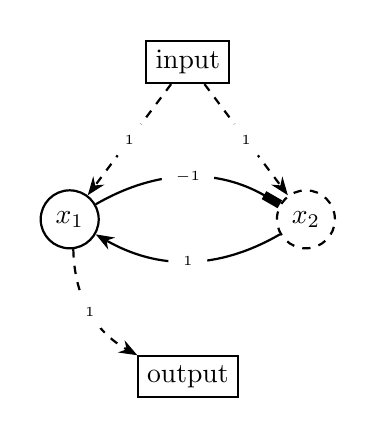
\begin{tikzpicture}[background rectangle/.style={fill=white}, show background rectangle]
            \begin{scope}[every node/.style={circle,thick,draw}]
              \node[black] (A) at (0,0) {$x_{1}$};
                \node[dashed, black] (B) at (3,0) {$x_{2}$};
                \node[shape=rectangle, black] (U) at (1.5,2) {input};
                \node[shape=rectangle, black] (y) at (1.5,-2) {output};
            \end{scope}

            \begin{scope}[>={Stealth[black]},
                          every node/.style={fill=white,circle},
                          every edge/.style={draw=black, thick}]
                \path [->, >=Rectangle] (A) edge[bend left] node {\tiny $-1$} (B);
                \path [->] (B) edge[bend left] node {\tiny $1$} (A); 
                \path[->] (U) edge[dashed] node {\tiny $1$} (A);
                \path[->] (U) edge[dashed] node {\tiny $1$} (B);
                \path[->] (A) edge[dashed,bend right] node {\tiny $1$} (y);
            \end{scope}
            \begin{scope}[>={Stealth[black]},
                          every edge/.style={draw=black, thick}]
                %\path [->] (A) edge[loop left] node {\tiny $\lambda_{1}$} (A);
                %\path [->] (B) edge[loop left] node {\tiny $\lambda_{2}$} (B);
            \end{scope}

            \end{tikzpicture}
        \end{center}
        \caption{
            Diagram of Example \ref{ex:osc} in the text.  
            \plr{explain what arrows mean if nec}
            \label{fig:oscillator_diagram}}
    \end{figure}
  \end{slide}

  \begin{slide}
    
    \begin{figure}
  \centering
  \begin{subfigure}{0.25\slideheight}
    \centering
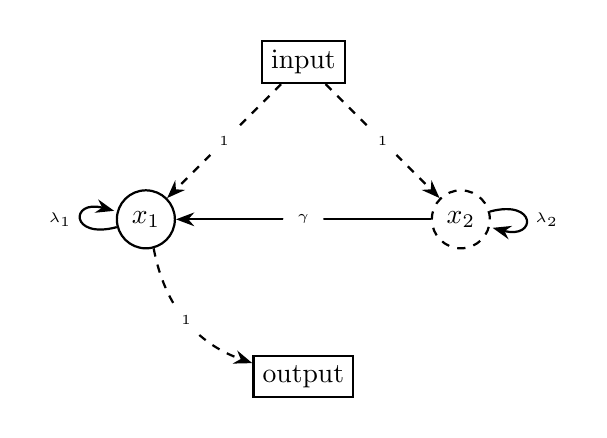
\begin{tikzpicture}[background rectangle/.style={fill=white}, show background rectangle]
\begin{scope}[every node/.style={circle,thick,draw}]
  \node[black] (A) at (0,0) {$x_{1}$};
    \node[dashed, black] (B) at (4,0) {$x_{2}$};
    \node[shape=rectangle, black] (U) at (2,2) {input};
    \node[shape=rectangle, black] (y) at (2,-2) {output};
\end{scope}

\begin{scope}[>={Stealth[black]},
              every node/.style={fill=white,circle},
              every edge/.style={draw=black, thick}]
    %\path [->] (A) edge[bend left] node {$c$} (B);
    \path [->] (B) edge node {\tiny $\gamma$} (A); 
    \path[->] (U) edge[dashed] node {\tiny $1$} (A);
    \path[->] (U) edge[dashed] node {\tiny $1$} (B);
    \path[->] (A) edge[dashed, bend right] node {\tiny $1$} (y);
\end{scope}
\begin{scope}[>={Stealth[black]},
              every edge/.style={draw=black, thick}]
    \path [->] (A) edge[loop left] node {\tiny $\lambda_{1}$} (A);
    \path [->] (B) edge[loop right] node {\tiny $\lambda_{2}$} (B);
\end{scope}

\end{tikzpicture}
    \caption{Gene Regulatory Network $A(0)$.}
  \end{subfigure}%
  \begin{subfigure}{0.25\slideheight}
    \centering
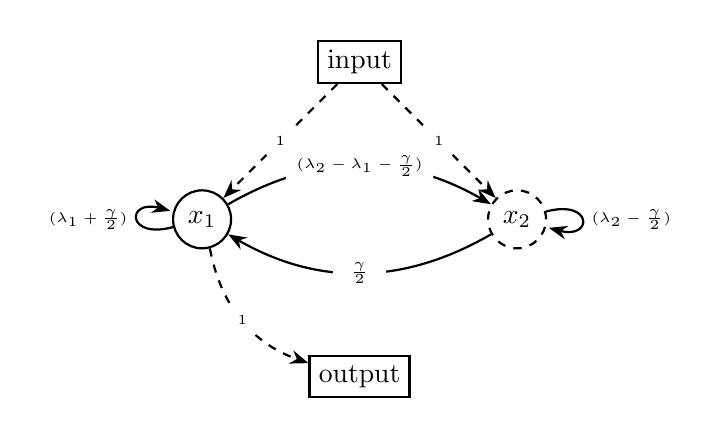
\begin{tikzpicture}[background rectangle/.style={fill=white}, show background rectangle]
\begin{scope}[every node/.style={circle,thick,draw}]
  \node[black] (A) at (0,0) {$x_{1}$};
    \node[dashed, black] (B) at (4,0) {$x_{2}$};
    \node[shape=rectangle, black] (U) at (2,2) {input};
    \node[shape=rectangle, black] (y) at (2,-2) {output};
\end{scope}

\begin{scope}[>={Stealth[black]},
              every node/.style={fill=white,circle},
              every edge/.style={draw=black, thick}]
    \path [->, sloped] (A) edge[bend left] node {\tiny $(\lambda_{2} - \lambda_{1} - \frac{\gamma}{2})$} (B);
    \path [->, sloped] (B) edge[bend left] node {\tiny $\frac{\gamma}{2}$} (A); 
    \path[->] (U) edge[dashed] node {\tiny $1$} (A);
    \path[->] (U) edge[dashed] node {\tiny $1$} (B);
    \path[->] (A) edge[dashed, bend right] node {\tiny $1$} (y);
\end{scope}
\begin{scope}[>={Stealth[black]},
              every edge/.style={draw=black, thick}]
    \path [->] (A) edge[loop left] node {\tiny $(\lambda_{1} + \frac{\gamma}{2})$} (A);
    \path [->] (B) edge[loop right] node {\tiny $(\lambda_{2}-\frac{\gamma}{2})$} (B);
\end{scope}

\end{tikzpicture}
    \caption{Gene Regulatory Network $A(-1)$.}
  \end{subfigure}
  \caption{Neutral rewiring of gene network $A(p)$ from Example \ref{ex:2x2}. Not only are the regulatory coefficients different between $A(0)$ and $A(-1)$, there is also a new regulatory connection.}
\end{figure}

\end{slide}
\end{document}
